% Chapter Template

\chapter{Method} % Main chapter title

\label{Chapter2} % Change X to a consecutive number; for referencing this chapter elsewhere, use \ref{ChapterX}

\lhead{\emph{Method}} % Change X to a consecutive number; this is for the header on each page - perhaps a shortened title

%----------------------------------------------------------------------------------------
%   SECTION 1
%----------------------------------------------------------------------------------------

\section{Initial Data}

In order to begin investigation into the phase diagrams of the CZTS system, which requires knowledge of the constituent Ternary phase diagrams (TPD) of the system; this, in turn requires knowledge of the three binary systems present in each TPD. As such, the binary phase diagrams for each of the element pairs, present in Appendix \ref{AppendixB} were examined in order to determine which compounds would be stable at a given temperature (initially 298K). Subsequently, data tables of the Gibbs Free energy, Enthalpy and Entropy for each of the elements and stable compounds were produced - Appendix \ref{AppendixA}. Further investigation into the temperature dependence of the Phase Diagrams of CZTS required reproduction of the data tables accounting for the change in temperature. 

%----------------------------------------------------------------------------------------
%   SECTION 2
%----------------------------------------------------------------------------------------

\section{Ternary Phase Diagrams}

Using the data found from the Binary phase diagrams, a set of four Ternary plots were constructed with a combination of the elements available in the system at the vertices, and the stable compounds of the elements at the vertices along the edges joining them. Each edge represents a percentage composition of the vertex element, with the stable compounds arranged accordingly. (INSERT EXAMPLE IMAGE)

%-----------------------------------
%   SUBSECTION 1
%-----------------------------------
\subsection{Tie-Lines}

Lines are then drawn from the stable compounds to the element at the opposite vertex, and the stable compounds on the other edges. These lines represent possible stable element-compound and compound-compound pairs - pairs of materials that could coexist at equilibrium. As the tie-lines are drawn, inevitably there will exist points where two will cross one another - these crossing points represent two possible equilibrium conditions, and can be summarised by a balanced reaction equation. 

%-----------------------------------
%   SUBSECTION 2
%-----------------------------------
\subsection{Method of Tie-Line Removal}

As the tie-lines are drawn, the ternary phase diagrams become congested and in order to reduce the congestion, the thermodynamically more favourable tie-line must be found. Calculation of the Gibb's Free Energy ($\Delta G_{r}^{\circ}$) of the reaction will yield the more favourable tie-line of the two; The Gibb's free energy is used as it is the maximum energy available for work, and as such when $\Delta G_{r}^{\circ}$ is minimum, the system is at equilibrium. Knowing this, by calculating $\Delta G_{r}^{\circ}$ for the reaction, using $\Delta G_{r}^{\circ} = \Sigma\Delta {G_{r}^{\circ}}_{products} - \Sigma\Delta {G_{r}^{\circ}}_{reactants}$, the more thermodynamically favourable of the two tie-lines is found, and the less favourable tie-line can be removed. Through repetition for each crossing point - only the favourable tie-lines remain, leaving no crossing points, and reducing the TPD to the stable phases.

%-----------------------------------
%   SUBSECTION 3
%-----------------------------------
\subsection{Examples}

\begin{figure}[ht]
\centering
\begin{subfigure}{80mm}
  \centering
    \includegraphics[width=80mm]{triangleplot_ZNSNS298-before.png}
    \caption{Before Calculations}
    \label{fig:ZnSnSBefore}
\end{subfigure}%
\begin{subfigure}{80mm}
 \centering
    \includegraphics[width=80mm]{triangleplot_ZNSNS298.png}
    \caption{After Calculations}
    \label{fig:ZnSnSAfter}
\end{subfigure}
\caption{Before and After Performing 'Tie-Line' Calculations. Percentage of each element run counter-clockwise.}
\label{fig:ZnSnSFigures}
\end{figure}

An example of the removal of tie-lines is examined below, starting from the example in \ref{fig:ZnSnSBefore}, and working towards that of \ref{fig:ZnSnSAfter}, the least favourable tie-lines are removed, leaving a diagram with no crossing points and thus the more favourable reactions.

\begin{enumerate}
\item For this point the balanced equation is 2 Zn + SnS$_2$ $\rightarrow$ 2 ZnS + Sn. $\Delta G_{r}^{\circ}$ for the reaction is found by: $\Delta G_{r}^{\circ} = (\Delta {G_{r}^{\circ}}_{ZnS} + \Delta {G_{r}^{\circ}}_{Sn}) - (\Delta {G_{r}^{\circ}}_{Zn} + \Delta {G_{r}^{\circ}}_{SnS_2})$. Using the data from the appendix, we find $\Delta G_{r}^{\circ}=(2\times-201.3 + 0)-(-145.5+2\times0)=$-257.1kJ mol$^{-1}$. Since the energy is found to be negative, the reaction moves left to right, as such we find that ZnS and Sn are in preference to Zn and SnS$_2$. As such the Zn and SnS$_2$ will be removed.

\item For this point the balanced equation is 3 ZnS + 2 Sn $\rightarrow$ 3 Zn + Sn$_2$S$_3$. $\Delta G_{r}^{\circ}$ for the reaction is found by $\Delta G_{r}^{\circ}=(2\times0 -245.3)-(3\times-201.3+2\times0)=$+358.6kJ mol$^{-1}$. We use the same method of calculation here to find that the ZnS and Sn should be retained whilst the Zn and Sn$_2$S$_3$ line discarded. 

\item For this point the balanced equation is Zn + SnS $\rightarrow$ ZnS + Sn. $\Delta G_{r}^{\circ}$ for the reaction is found by: $\Delta G_{r}^{\circ}=(0+ -201.3)-(-98.3+0)$-257.1kJ mol$^{-1}$. Using the same method as before we find that the ZnS and Sn line should remain.
\item This point and points 5 and 6 no longer occur due to the removal of less favoured tie-lines at points 1-3. 
\end{enumerate}

%----------------------------------------------------------------------------------------
%   SECTION 3
%----------------------------------------------------------------------------------------

\section{Quaternary Phase Diagrams}

Upon determination of the four ternary phase diagrams, a quaternary phase diagram may be constructed, by joining each of the TPD's on their common edges to form a tetrahedron. On the faces of the Quaternary Diagram will exist the stable phases present on the reduced ternary phase diagrams, and in some cases the joining of the tie-lines may form an internal plane or 'tie-phase'. Dependent upon the positioning of these 'tie-phases' within the quaternary diagram, they may be candidates for the quasi-ternary diagram for CZTS,an example of which is demonstrated by \ref{fig:ZnSSnSCu} - this figure demonstrates the Quasi-TPD with stable compounds at the vertices. In order to calculate whether a 'tie-phase' is a candidate for  the Thermodynamic location of CZTS, it must firstly contain the correct ratio of Sulphur to the other three elements. 

\begin{figure}[ht]
\centering
    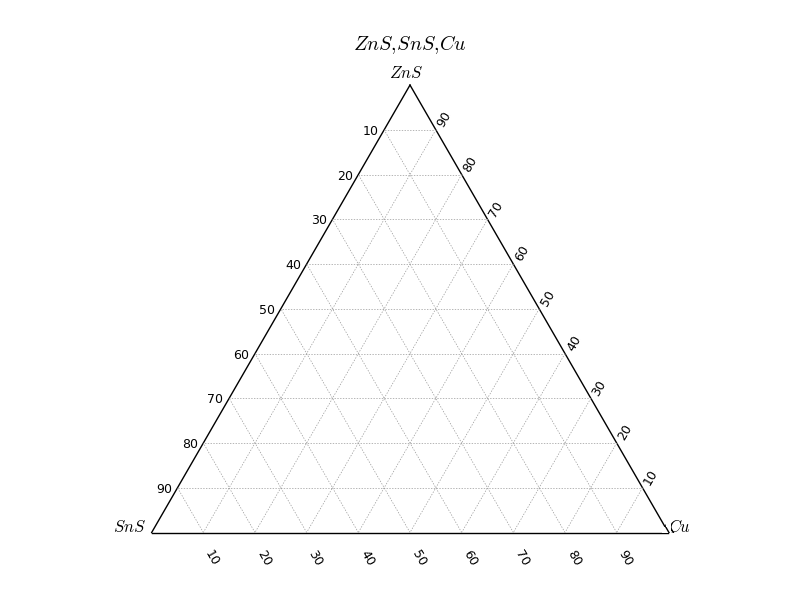
\includegraphics[width=130mm]{triangleplot_ZnSSnSCu298.png}
\caption{Dismissed tie Phase Diagram, without associated phases}
\label{fig:ZnSSnSCu}
\end{figure}


%----------------------------------------------------------------------------------------
%   SECTION 4
%----------------------------------------------------------------------------------------

\section{Quasi-Ternary Phase Diagrams}

Once the 'tie-phase' with the correct ratio of elements has been identified, one can construct a Quasi-Ternary Diagram describing the Primary and Secondary phases, as well as the Thermodynamic location of CZTS.

